\documentclass[11pt, oneside]{article}   	% use "amsart" instead of "article" for AMSLaTeX format
\usepackage{geometry}                		% See geometry.pdf to learn the layout options. There are lots.
\geometry{letterpaper}                   		% ... or a4paper or a5paper or ... 
%\geometry{landscape}                		% Activate for for rotated page geometry
%\usepackage[parfill]{parskip}    		% Activate to begin paragraphs with an empty line rather than an indent
\usepackage{graphicx}				% Use pdf, png, jpg, or eps with pdflatex; use eps in DVI mode
								% TeX will automatically convert eps --> pdf in pdflatex		
\usepackage{amssymb}
\graphicspath{{/Users/telliott_admin/Dropbox/Tex/png/}}

\title{Induction}
%\author{The Author}
\date{}							% Activate to display a given date or no date

\begin{document}
\large
\maketitle
%\section{}
%\subsection{}
In the figure below we have a polygon---an irregular heptagon.  Actually, there are two polygons, there is the heptagon with $n+1$ sides, and also the hexagon with only $n$ sides that would result from cutting along the dotted line.
\begin{center}
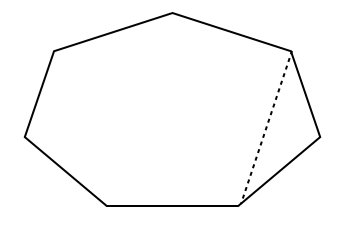
\includegraphics [scale=0.5] {polygon.png}
\end{center}
What we would like to do is to find a formula for the sum of the internal angles that depends only on the number of sides or vertices.

The first part of the answer is to guess.  In the figure, you can see that by adding the extra vertex to go to the $n+1$-gon, we added a triangle, or perhaps you'd rather say than in going from $n+1$ to $n$ we lost a triangle.  In either case, the difference is $180^\circ$.  The difference between having $n$ sides and $n+1$ sides is to add $180^\circ$.  The second part of the argument is to suppose that $n=3$, in that case we must have simply $180^\circ$ degrees for a triangle.  So we guess that the formula may be
\[ (n-2)180^\circ = S_n \]
where S is the sum of the angles in an $n$-gon.
We can use induction to prove that this formula is correct.

Actually, we've already done the inducing part of induction, when we guessed the formula and verified it for one or a few cases.  Now we'd like to actually prove it.  The proof has two parts.  We must verify the formula for a base case like the triangle, which we've done.  You may wish to check that it works for the square as well, but that's not necessary.

The second part of the proof is to verify that in going from $n$ to $n+1$, we add another $180^\circ$.  \[ (n-2)180^\circ + 180^\circ \stackrel{?}{=} (n-1)180^\circ \]
On the left-hand side, we have the sum of angles for $n$ sides, which we assume is correct, and then we just add $180^\circ$ to it.  On the right, we have substituted $n+1$ into the formula $((n+1)-2=n-1)$.  Now we need to show that these are equivalent.
But of course
\[ (n-2)x + x = nx - 2x + x = nx + (-2 + 1)x = nx - x = (n-1) x \]
QED.
\vspace{2 mm}

That is the inductive proof of the formula.

We can visualize an inductive proof as a kind of chain.  We know that the "base case" is true, say for n = 3.  We also know that if the formula works for n, it must work for n+1.
\vspace{2mm}

We know it works for $n = 3$;  therefore it works for $n = 4$
\vspace{2mm}

We know it works for $n = 4$;  therefore it works for $n = 5$
\vspace{2mm}

We know it works for $n = 5$;  therefore it works for $n = 6 \cdots$
\vspace{2mm}

Another famous example of induction is in the proof of the formula for the sum of the integers from $1$ to $n$
\[  1 + 2 + 3 + \cdots + n = ?  \]
There is a famous story about Gauss that (in the simplified version) he "saw" how to add the integers from $1$ to $100$ as two parallel sums
\[  \ 1 \ + \ 2 + \ 3 + \cdots + \ 99 + 100 \]
\[ 100 + 99 + 98 + \cdots + 2 + 1 \]
Added together horizontally, these two series equal the sum of $1:100$.  But notice that we have $n$ sums vertically, each of which is equal to $n+1$.  We induce that
\[ 2S_n = n (n+1), \ \ \ \  S_n = \frac{1}{2}n(n+1)\]
The proof follows the inductive method.  We first check that the formula gives the correct answer for n = 1, say.  
And then we add $n+1$ to $S_n$:
\[ \frac{1}{2} n (n+1) + (n+1) \]
\[ \frac{1}{2} n (n+1) + \frac{1}{2} (2) (n+1) \]
\[ \frac{1}{2}[n(n+1) + 2(n+1)] \]
\[ \frac{1}{2}(n+2)(n+1) = S_{n+1}\]
QED.
\vspace{2mm}

Another formula that you'll see used (particularly in introducing integration) is the sum of squares of the integers 
\[ \sum_{k=1}^{n} \ k^2 = 1^2 + 2^2 + 3^2 + \cdots + n^2 \]
\[ \frac{n(n+1)(2n+1)}{6} \]
This is harder to guess, but having somehow done so, we can check the base case
\[ n = 2, 1^2 + 2^2 = 5 = \frac{(2)(3)(5)}{6} \]
The other step is 
\[ \frac{n(n+1)(2n+1)}{6} + (n+1)^2 \]
\[ \frac{[n(n+1)(2n+1) + 6(n+1)^2]}{6} \]
Factor out an $(n+1)$
\[ \frac{(n+1) \ [n(2n+1) + 6(n+1)]}{6} \]
\[ \frac{(n+1)(2n^2 + 7n + 6)}{6} \]
\[ \frac{(n+1)(n+2)(2n+3)}{6} \]
\[ \frac{(n+1)[(n+1)+1][2(n+1)+1]}{6} \]
But this is just our formula, with $n+1$.

\noindent QED.


\end{document}  